\documentclass[brazil, notheorems, 10pt]{beamer}
%
%   Arquivo de Configuração dos Slides
%


%
%   Pacotes utilizados
%

% Codificação dos caracteres em formato universal.
\usepackage[utf8]{inputenc}
\usepackage[T1]{fontenc}

% Traduz o texto gerados pelo LaTeX para português. ex.: Capítulo, Seção, Conteúdo.
\usepackage[brazil]{babel}

% Pacotes para ambientes matemáticos
\usepackage{amsmath}
\usepackage{amsthm}
\usepackage{amssymb}

% Diversas funções para o uso das aspas.
\usepackage{csquotes}

% Outros pacotes
\usepackage{hyperref}
\usepackage{tikz}
\usepackage{yfonts}
\usepackage{colortbl}
\usepackage{ragged2e}
\usepackage{helvet}
\usepackage{verbatim}


%
%   Tema
%

% Copyright 2007 by Till Tantau
%
% This file may be distributed and/or modified
%
% 1. under the LaTeX Project Public License and/or
% 2. under the GNU Public License.
%
% See the file doc/licenses/LICENSE for more details.


% Common packages


\usepackage[brazil]{babel}
\usepackage[utf8]{inputenc}
\usepackage{times}
 \mode<article> {
  \usepackage{times}
  \usepackage{mathptmx}
  \usepackage[left=1.5cm,right=6cm,top=1.5cm,bottom=3cm]{geometry}
}

\usepackage{hyperref}
\usepackage[T1]{fontenc}
\usepackage{amsmath,amssymb}
\usepackage{tikz}
\usepackage{colortbl}
\usepackage{yfonts}
\usepackage{colortbl}
\usepackage{translator} % comment this, if not available
\usepackage{ragged2e} % justifying
% Or whatever. Note that the encoding and the font should match. If T1
% does not look nice, try deleting the line with the fontenc.
\usepackage{helvet}
\usepackage{verbatim}


%\usepackage{lipsum}
%\usepackage{enumitem}


\usetheme[
%%% options passed to the outer theme
%    hidetitle,           % hide the (short) title in the sidebar
%    hideauthor,          % hide the (short) author in the sidebar
%    hideinstitute,       % hide the (short) institute in the bottom of the sidebar
%    shownavsym,          % show the navigation symbols
%    width=2cm,           % width of the sidebar (default is 2 cm)
%    hideothersubsections,% hide all subsections but the subsections in the current section
%    hideallsubsections,  % hide all subsections
    right               % right of left position of sidebar (default is right)
%%% options passed to the color theme
%    lightheaderbg,       % use a light header background
  ]{AAUsidebar}

% If you want to change the colors of the various elements in the theme, edit and uncomment the following lines
% Change the bar and sidebar colors:
%\setbeamercolor{AAUsidebar}{fg=red!20,bg=red}
%\setbeamercolor{sidebar}{bg=red!20}
% Change the color of the structural elements:
%\setbeamercolor{structure}{fg=red}
% Change the frame title text color:
%\setbeamercolor{frametitle}{fg=blue}
% Change the normal text color background:
%\setbeamercolor{normal text}{bg=gray!10}
% Highlight the text in the sidebar
\usecolortheme{rose,sidebartab}
% ... and you can of course change a lot more - see the beamer user manual.

% colored hyperlinks
\newcommand{\chref}[2]{%
  \href{#1}{{\usebeamercolor[bg]{AAUsidebar}#2}}%
}


\newcommand{\prn}[1]{\left(#1\right)}

% specify a logo on the titlepage (you can specify additional logos an include them in
% institute command below
\pgfdeclareimage[height=1cm]{titlepagelogo}{theme/figures/ufrn2} % placed on the title page
\pgfdeclareimage[height=1cm]{titlepagelogo2}{theme/figures/imd} % placed on the title page
\titlegraphic{% is placed on the bottom of the title page
  \pgfuseimage{titlepagelogo}
  \hspace{1cm}\pgfuseimage{titlepagelogo2}
}


% Article version layout settings

\mode<article>

\makeatletter
\def\@listI{\leftmargin\leftmargini
  \parsep 0pt
  \topsep 5\p@   \@plus3\p@ \@minus5\p@
  \itemsep0pt}
\let\@listi=\@listI


\setbeamertemplate{frametitle}{\paragraph*{\insertframetitle\
    \ \small\insertframesubtitle}\ \par
}
\setbeamertemplate{frame end}{%
  \marginpar{\scriptsize\hbox to 1cm{\sffamily%
      \hfill\strut\insertshortlecture.\insertframenumber}\hrule height .2pt}}
\setlength{\marginparwidth}{1cm}
\setlength{\marginparsep}{4.5cm}

\def\@maketitle{\makechapter}

\def\makechapter{
  \newpage
  \null
  \vskip 2em%
  {%
    \parindent=0pt
    \raggedright
    \sffamily
    \vskip8pt
    
\includegraphics[width=\linewidth]{theme/figures/imd.png}\par\vskip2em
    {\fontsize{36pt}{36pt}\selectfont Aula \insertshortlecture \par\vskip2pt}
    {\fontsize{24pt}{28pt}\selectfont \color{blue!50!black} \@title\par\vskip4pt}
    %{\Large\selectfont \color{blue!50!black} \insertsubtitle\par}
    \vskip10pt

    \normalsize\selectfont [Notas de Aula]
    Disciplina: \emph{\lecturename \ (\semestre)} \par\vskip1.5em
    \nomedoautor\hskip1em Email: \ \emaildoautor
  }
  \par
  \vskip 1.5em%
}

\let\origstartsection=\@startsection
\def\@startsection#1#2#3#4#5#6{%
  \origstartsection{#1}{#2}{#3}{#4}{#5}{#6\normalfont\sffamily\color{blue!50!black}\selectfont}}

\makeatother

\mode
<all>




% Typesetting Listings

\usepackage{listings}
\lstset{language=Java}

\alt<presentation>
{\lstset{%
  basicstyle=\footnotesize\ttfamily,
  commentstyle=\slshape\color{green!50!black},
  keywordstyle=\bfseries\color{blue!50!black},
  identifierstyle=\color{blue},
  stringstyle=\color{orange},
  escapechar=\#,
  emphstyle=\color{red}}
}
{
  \lstset{%
    basicstyle=\ttfamily,
    keywordstyle=\bfseries,
    commentstyle=\itshape,
    escapechar=\#,
    emphstyle=\bfseries\color{red}
  }
}



% Common theorem-like environments
%\usepackage{amsthm}

\setbeamertemplate{theorems}[numbered]

\theoremstyle{plain}
\newtheorem{Teo}{Teorema}


\theoremstyle{definition}

\newtheorem{Def}[Teo]{Definição}
\newtheorem{exercise}{Exercício}

\theoremstyle{remark}

\newtheorem{Obs}[Teo]{Observação}




\newtheorem{Exer}[Teo]{Exercicio Resolvido}%{\translate{Exercise}}

\newtheorem{Cor}[Teo]{Corolário}
\newtheorem{Exem}[Teo]{Exemplo}
\newtheorem{Lem}[Teo]{Lema}
\newtheorem{Prop}[Teo]{Proposição}
\newtheorem{Sumario}[Teo]{Sumário}
\newtheorem{Obse}{Observação}

\newcounter{Listaexercicios}
\def\Ex#1{
\stepcounter{Listaexercicios} \textbf{\arabic{Listaexercicios}}. #1
}




% New useful definitions:

\newbox\mytempbox
\newdimen\mytempdimen

\newcommand\includegraphicscopyright[3][]{%
  \leavevmode\vbox{\vskip3pt\raggedright\setbox\mytempbox=\hbox{\includegraphics[#1]{#2}}%
    \mytempdimen=\wd\mytempbox\box\mytempbox\par\vskip1pt%
    \fontsize{3}{3.5}\selectfont{\color{black!25}{\vbox{\hsize=\mytempdimen#3}}}\vskip3pt%
}}

\newenvironment{colortabular}[1]{\medskip\rowcolors[]{1}{blue!20}{blue!10}\tabular{#1}\rowcolor{blue!40}}{\endtabular\medskip}

\def\equad{\leavevmode\hbox{}\quad}

\newenvironment{greencolortabular}[1]
{\medskip\rowcolors[]{1}{green!50!black!20}{green!50!black!10}%
  \tabular{#1}\rowcolor{green!50!black!40}}%
{\endtabular\medskip}

%\setbeamertemplate{theorem begin}{{ \inserttheoremheadfont
%\inserttheoremname \inserttheoremnumber
%\ifx\inserttheoremaddition\empty\else\ (\inserttheoremaddition)\fi%
%\inserttheorempunctuation }} \setbeamertemplate{theorem end}{}

\newcommand{\vu}{\vec{u}}
\newcommand{\vv}{\vec{v}}
\newcommand{\vi}{\vec{i}}
\newcommand{\vj}{\vec{j}}
\newcommand{\vk}{\vec{k}}
\newcommand{\vw}{\vec{w}}
\newcommand{\R}{\mathbb{R}}
\newcommand{\N}{\mathbb{N}}
\newcommand{\Z}{\mathbb{Z}}
\newcommand{\Q}{\mathbb{Q}}
\newcommand{\C}{\mathbb{C}}
\newcommand{\U}{\mathcal U}
\newcommand{\I}{\mathcal I}
\newcommand{\sen}{\text{sen}}
\newcommand\seg[2]{\overline{#1#2}}
\def\set#1{\left\{#1\right\}}
\def\paren#1{\left(#1\right)}
\def\colc#1{\left[#1\right]}
\def\modu#1{\left|#1\right|}
\def\tq{\;;\;}
\def\sub#1{\underline{#1}}
\def\link#1#2{\href{#1}{{\tt #2}}}



%
%   Macros
%

\usepackage{macros/macros}


%
%   Ambientes
%

\theoremstyle{plain}
\newtheorem{teorema}{Teorema}

\theoremstyle{definition}
\newtheorem{definicao}[teorema]{Definição}
%\newtheorem{exercicio}{Exercício}

\theoremstyle{remark}
\newtheorem{obs}[teorema]{Observação}
\newtheorem{observacao}[teorema]{Observação}
\newtheorem{corolario}[teorema]{Corolário}
\newtheorem{exemplo}[teorema]{Exemplo}
\newtheorem{lema}[teorema]{Lema}
\newtheorem{proposicao}[teorema]{Proposição}

\newcounter{exercicios}
\newenvironment{exercicio}{\stepcounter{exercicios} \textbf{\arabic{exercicios}}.}{}

% compatibilidade
\newcommand{\Ex}[1]{\begin{exercicio}#1\end{exercicio}}

%
%   Definições e comandos auxiliares do preâmbulo
%

\newcommand{\capitulo}[1]{\lecture[#1]{Capítulo}}
\newcommand{\aula}[1]{\subtitle{#1}}
\newcommand{\autor}{Igor Oliveira}
\newcommand{\email}{\href{mailto:matematicaelementar@imd.ufrn.br}{\texttt{matematicaelementar@imd.ufrn.br}}}
\newcommand{\disciplina}{Matemática Elementar}
\newcommand{\codigo}{IMD1001}

\title{\disciplina}
\date{\today}
\author[\autor]
{
    \autor\\
    \email
}

\def\lecturename{\codigo

\disciplina}

\institute[
	UFRN\\
	Natal-RN
]
{
	Instituto Metrópole Digital\\
	Universidade Federal do Rio Grande do Norte\\
	Natal-RN

}

% compatibilidade
\newcommand{\vu}{\vec{u}}
\newcommand{\vv}{\vec{v}}
\newcommand{\vi}{\vec{i}}
\newcommand{\vj}{\vec{j}}
\newcommand{\vk}{\vec{k}}
\newcommand{\vw}{\vec{w}}
\newcommand{\segmento}[2]{\overline{#1#2}}
\def\colc#1{\left[#1\right]}
\newcommand{\negacao}{\sim}

\justifying



%lecture[number of class]{type}
\lecture[9]{Capítulo}

\def\lecturename{IMD1001
Matemática Elementar}
\def\semestre{2018.1}
\def\nomedoautor{Igor Oliveira}
\def\emaildoautor{\href{mailto:igoroliveira@imd.ufrn.br}{{\tt igoroliveira@imd.ufrn.br}}}

\title[\lecturename]% optional, use only with long paper titles
{Matemática Elementar}

\subtitle{Funções Exponenciais e Logarítmicas}  % could also be a conference name

\date{\today}

\author[Igor Oliveira] % optional, use only with lots of authors
{
	\nomedoautor\\
	\emaildoautor
}
% - Give the names in the same order as they appear in the paper.
% - Use the \inst{?} command only if the authors have different
%   affiliation. See the beamer manual for an example

\institute[
%  {\includegraphics[scale=0.2]{aau_segl}}\\ %insert a company, department or university logo
	UFRN\\
	Natal-RN
] % optional - is placed in the bottom of the sidebar on every slide
{% is placed on the title page
	Instituto Metrópole Digital\\
	Universidade Federal do Rio Grande do Norte\\
	Natal-RN

	%there must be an empty line above this line - otherwise some unwanted space is added between the university and the country (I do not know why;( )
}


\begin{document}

\mode<article>
{
\begin{frame} % the plain option removes the sidebar and header from the title page
	\maketitle
\end{frame}

% the titlepage
\begin{frame}[plain,noframenumbering] % the plain option removes the sidebar and header from the title page
	\titlepage
\end{frame}
}

\mode<presentation>
{
% the titlepage
{\imagemfundo
\begin{frame}[plain,noframenumbering] % the plain option removes the sidebar and header from the title page
	\titlepage
\end{frame}}
}

% TOC
\begin{frame}{Índice}{}
\tableofcontents
\end{frame}
%%%%%%%%%%%%%%%%


\section{Introdução}

\begin{frame}  \frametitle{Apresentação da Aula}

As funções do tipo exponenciais modelam problemas nos quais o crescimento
é calculado dependendo do valor no momento anterior, como em juros
compostos. Por que será que a expressão ``crescimento exponencial''
é sinônimo de um crescimento muito acentuado?

Além disso, a função exponencial é a única função real contínua que
transforma somas em produtos, ou seja, $$f(x+y) = f(x) \cdot f(y).$$

A função logarítmica, \emph{que será apresentada na segunda parte
desse capítulo}, é a inversa da função exponencial. Por isso,
teremos que ela é a única função real contínua que transforma
produtos em somas, ou seja,
$$f(xy) = f(x) + f(y).$$


\end{frame}


%------------------------------------------------------------------------------------------------------------

\begin{comment}
\section{Objetivos}
\frame
{
\frametitle{Objetivos}

\begin{itemize}
\item<1-> Conhecer os \alert{sinais analógicos} e digitais
\item<2-> Fazer uma comparação entre sistemas analógicos e digitais
\item<3-> Conhecer os elementos elétricos passivos : resistor, capacitor e indutor
\item<4-> Conhecer as Leis de Kirchhoff
\item<5-> Conhecer os transistores e os diodos
\item<6-> Analisar as principais aplicações de sistemas digitais.
\end{itemize}

}
\end{comment}

%------------------------------------------------------------------------------------------------------------

\section{Função Exponencial}
\begin{frame} \frametitle{Definição}
\begin{Def}
Seja $a$ um número real positivo diferente de 1. Chamamos de
\sub{função exponencial} uma função $f: \R \to \R_+^\ast$ com lei de
formação $f(x) =
 a^x$. O número $a$ é chamado de \sub{base} da função exponencial.
\end{Def}\pause



\begin{Def}
Dizemos que uma função $f: \R \to \R$ é de \sub{tipo exponencial}
quando $f(x) =b\cdot a^x$, onde $a,b \in\R$, $b$ é não nulo e $a$ é
positivo e diferente de 1.
\end{Def}





\end{frame}

%------------------------------------------------------------------------------------------------------------

\begin{frame}
\frametitle{Propriedades} %\framesubtitle{Exemplos}

\begin{Prop}[Propriedades Fundamentais da Função Exponencial]
Seja $f: \R \to \R_+^\ast$ uma função exponencial de base $a$.
Então, para quaisquer $x, y \in \R$ valem:
\begin{enumerate}[(i)]
	\item  $a^{x+y} = a^x\cdot a^y$, ou seja, $f(x+y) = f(x)\cdot f(y)$;
	\item $a^1 = a$, ou seja, $f(1) = a$;
	\item $x<y \implies \begin{cases} a^x < a^y, \ \ \ \text{ quando } \ \ \ a>1 \\
																		a^y < a^x, \ \ \ \text{ quando } \ \ \ 0<a<1
											 \end{cases}.$
\end{enumerate}
\end{Prop}




\end{frame}

%------------------------------------------------------------------------------------------------------------

\begin{frame}
\frametitle{Propriedades} %\framesubtitle{Exemplos}

Devido a essas propriedades, podemos concluir os seguintes
resultados acerca de uma função exponencial $f: \R \to \R_+^\ast$:
\begin{itemize}
	\item $f^{-1}(0) = \emptyset$, ou seja, $f$ não pode assumir o valor
	zero;
	\item $f(x)>0$, para todo $x \in \R$;
	\item Ao escolhermos o conjunto $\R_+^\ast$ como contradomínio de $f$, obtemos
	a sobrejetividade da função;
	\item $f$ é ilimitada superiormente;
	\item O gráfico de $f$ é uma linha contínua;
	\item $f$ é bijetiva e crescente se $a>1$, ou decrescente se
	$0<a<1$.
\end{itemize}
\end{frame}



%------------------------------------------------------------------------------------------------------------
\section{Gráfico da Função Exponencial}
\begin{frame}
\frametitle{Gráfico da Função Exponencial} %\framesubtitle{Exemplos}

\begin{Exem}
Seja $f: \R \to \R_+^\ast$ uma função exponencial tal que $f(x) =
a^x$. O gráfico de $f$ é:
\begin{center}
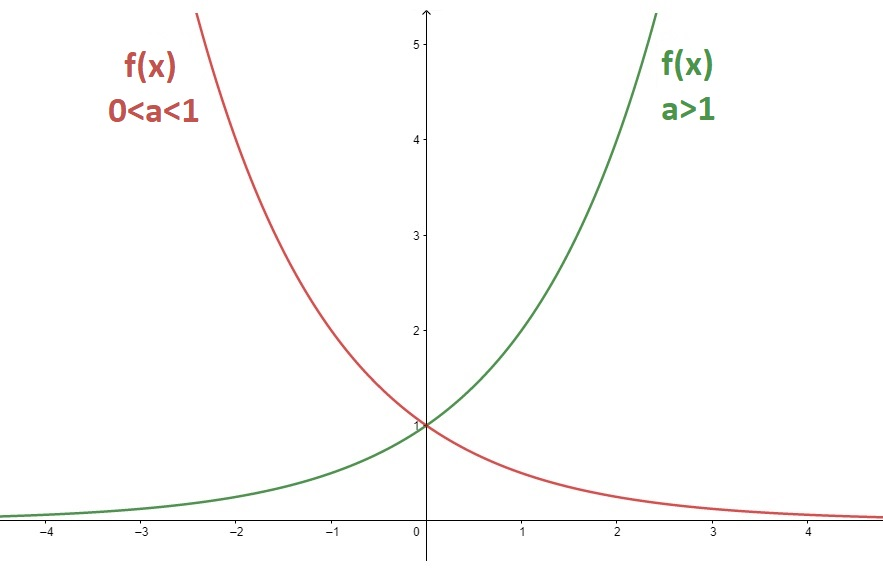
\includegraphics[width=6.3cm]{figures/grafexp.jpg}
\end{center}
O gráfico de $f$ nunca toca o eixo $x$, mas fica tão próximo quanto
queiramos. Isso equivale dizer que a reta $y=0$ é \sub{assíntota} do
gráfico de $f$.
\end{Exem}

\end{frame}



%------------------------------------------------------------------------------------------------------------

\begin{frame}
\frametitle{Gráfico da Função Exponencial} %\framesubtitle{Exemplos}

\begin{Exem}
O crescimento exponencial supera o de qualquer polinômio. Ao
compararmos, por exemplo, as funções $f(x) = 2^x$ e
$p(x)=x^{10}$, temos que:\\
\begin{tabular}{ccc}
$0<x<1{,}077$ & $\implies$ & $2^x > x^{10}$\\
$1{,}077 < x < 58{,}77$ & $\implies$ & $x^{10} > 2^x$\\
$x>58{,}77$ & $\implies $& $2^x > x^{10}$
\end{tabular}
\begin{center}
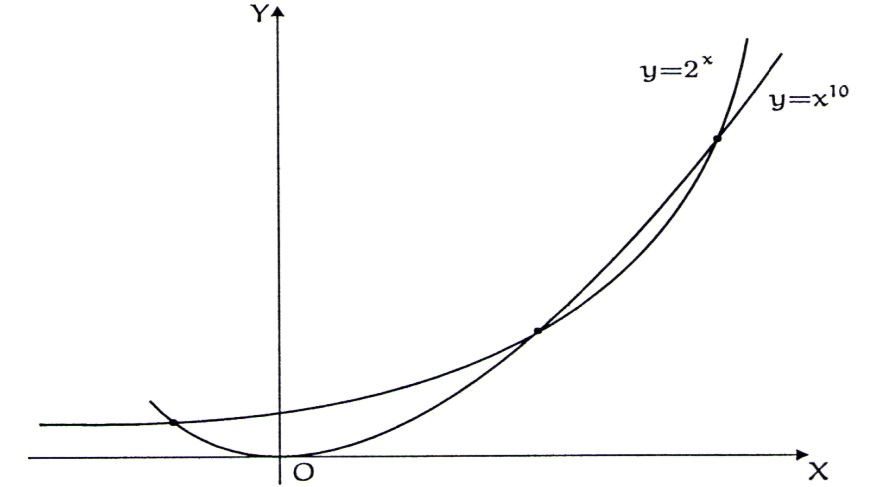
\includegraphics[width=7cm]{figures/polXexp.jpg}
\end{center}
\end{Exem}

\end{frame}

%------------------------------------------------------------------------------------------------------------
\section{Atividade Online}
\begin{frame}
\frametitle{Atividade Online} %\framesubtitle{Exemplos}


\href{https://pt.khanacademy.org/math/algebra/introduction-to-exponential-functions/exponential-expressions-alg1/e/exponential-expressions-word-problems-algebraic}
{{\tt Atividade 10 - Problemas (Algébricos) de Expressões
Exponenciais}}

%\href{https://pt.khanacademy.org/math/algebra/introduction-to-exponential-functions/graphs-of-exponential-growth/e/graphing-exponential-growth-intro}
%{{\tt Atividade 11 - Gráficos de Crescimento Exponencial}}

%\href{https://pt.khanacademy.org/math/algebra/introduction-to-exponential-functions/exponential-decay-alg1/e/exponential-growth-vs-decay}
%{{\tt Atividade 12 - Crescimento Versus Decaimento Exponencial}}

\href{https://pt.khanacademy.org/math/algebra/introduction-to-exponential-functions/exponential-decay-alg1/e/graphs-of-basic-exponential-functions}
{{\tt Atividade 11 - Representação Gráfica de Crescimento e
Decaimento Exponencial}}

%\href{https://pt.khanacademy.org/math/algebra/introduction-to-exponential-functions/exponential-functions-from-tables-and-graphs/e/construct-basic-exponential-functions-from-table-or-graph}
%{{\tt Atividade 14 - Funções Exponenciais com Base em Tabelas e
%Gráficos}}

Veja o desempenho na Missão Álgebra I.

\href{https://pt.khanacademy.org/math/algebra2/exponential-and-logarithmic-functions/graphs-of-exponential-functions/e/graphs-of-exponential-functions}
{{\tt Atividade 12 - Gráficos de Funções Exponenciais}}

Veja o desempenho na Missão Álgebra II.
\end{frame}
%------------------------------------------------------------------------------------------------------------
\section{Caracterização da Função Exponencial}
\begin{frame}
\frametitle{Caracterização da Função Exponencial} %\framesubtitle{Exemplos}

\begin{Teo}[Caracterização da Função Exponencial]
Seja $f: \R \to \R_+^\ast$ uma função monótona injetiva. As
seguintes afirmações são equivalentes:
\begin{enumerate}[(i)]
	\item $f(nx) = f(x)^n$ para todo $n \in \Z$ e todo $x \in \R$;
	\item $f(x) = a^x$ para todo $x\in \R$, onde $a = f(1)$;
	\item $f(x+y) = f(x)\cdot f(y)$ para quaisquer $x, y \in \R$.
\end{enumerate}
\end{Teo}



\end{frame}

%------------------------------------------------------------------------------------------------------------
\section{Funções Exponenciais e Progressões}
\begin{frame}
\frametitle{Funções Exponenciais e Progressões} %\framesubtitle{Exemplos}

\begin{Prop}
Seja  $f: \R \to \R$. Se $f$ é uma função do tipo exponencial e
$\paren{x_1, x_2, \dots , x_i, \dots}$ é uma PA, então a sequência
formada pelos pontos $y_i = f(x_i)$, $i \in \N^{\ast}$ é uma PG.
Reciprocamente, se $f$ for monótona injetiva e transformar qualquer
PA $\paren{x_1, x_2, \dots , x_i, \dots}$ numa PG com termo geral
$y_i = f(x_i)$, $i \in \N^{\ast}$ então $f$ é uma função real tal
que $f(x) = b \cdot a^x$ com $b = f(0)$ e $a = \frac {f(1)} {f(0)}$.
\end{Prop}

\end{frame}




%------------------------------------------------------------------------------------------------------------
\section{Função Logarítmica}
\begin{frame}
\frametitle{Definição} %\framesubtitle{Exemplos}
\begin{Def}
A inversa da função exponencial de base $a$ é a \sub{função
logarítmica}
$$\log_a : \R_+^\ast \to \R,$$
que associa a cada número real positivo $x$ o número real $\log_a
x$, chamado \sub{logaritmo} de $x$ na base $a$. No caso de $a=10$,
escrevemos, por simplicidade, $\log_{10}x = \log
 x$.
\end{Def}\pause
Pela definição de função inversa, tem-se
$$ a^{\log_a x}=x \ \ \ \text{ e } \ \ \ \log_a \paren{a^x} = x.$$
Assim, $\log_a x $ é o expoente ao qual se deve elevar a base $a$
para obter o número $x$. Ou seja,
$$ y = \log_a x \iff a^y = x.$$

\end{frame}


%------------------------------------------------------------------------------------------------------------
\begin{frame}
\frametitle{Propriedades} %\framesubtitle{Exemplos}

\begin{Prop}
Seja $f: \R_+^\ast \to \R$ uma função logarítmica tal que $f(x) =
\log_a x$. Os seguintes valem para quaisquer  $x, y, b \in
\R_+^\ast$, $b \neq 1$ e qualquer $k \in \R$:
\begin{enumerate}[(a)]
	\item $\log_a \paren{xy} = \log_a x + \log_a y$;
	\item $\log_a x^k = k\cdot \log_a x$;
	\item $\log_a 1 = 0$;
	\item $\log_a x = \frac{\log_b x}{\log_b a}$;
	\item $f$ é bijetiva com contradomínio $\R$, logo é ilimitada superiormente e inferiormente;
	\item O gráfico de $f$ é traçado por uma linha contínua;
	\item $f$ é crescente se $a>1$ e decrescente se $0<a<1$.
\end{enumerate}
\end{Prop}


\end{frame}
%------------------------------------------------------------------------------------------------------------
\section{Atividade Online}
\begin{frame}
\frametitle{Atividade Online} %\framesubtitle{Exemplos}

\href{https://pt.khanacademy.org/math/algebra2/exponential-and-logarithmic-functions/introduction-to-logarithms/e/logarithms_1.5}
{{\tt Atividade 13 - Cálculo de Logaritmos (Avançado)}}

\href{https://pt.khanacademy.org/math/algebra2/exponential-and-logarithmic-functions/properties-of-logarithms/e/logarithms_2}
{{\tt Atividade 14 - Use as Propriedades dos Logaritmos }}

\href{https://pt.khanacademy.org/math/algebra2/exponential-and-logarithmic-functions/change-of-base-formula-for-logarithms/e/rewrite-logarithmic-expressions-using-the-change-of-base-rule}
{{\tt Atividade 15 - Use a Regra da Mudança de Base dos Logaritmos}}

Veja o desempenho na Missão Álgebra II.


\end{frame}
%------------------------------------------------------------------------------------------------------------

\section{Gráfico da Função Logarítmica}
\begin{frame}
\frametitle{Gráfico da Função Logarítmica} %\framesubtitle{Exemplos}

\begin{Exem}
Considere as funções logarítmicas tais que $f(x) = \log_2 x$ e $g(x)
= \log_{\frac 1 2} x$. Os gráficos de $f$ e $g$ são apresentados
abaixo.
\begin{center}
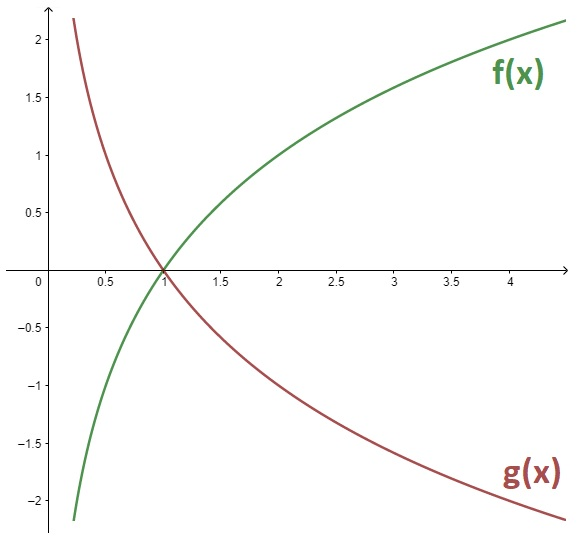
\includegraphics[width=6.1cm]{figures/graflog.jpg}
\end{center}
\end{Exem}


\end{frame}

%------------------------------------------------------------------------------------------------------------

\begin{frame}
\frametitle{Gráfico da Função Logarítmica} %\framesubtitle{Exemplos}


Já vimos que o crescimento exponencial supera o de qualquer
polinômio. Por ser a inversa da função exponencial, a função
logarítmica possui um crescimento muito lento. Mesmo assim, a função
logarítmica é ilimitada superiormente. Compare os gráficos abaixo:
\begin{center}
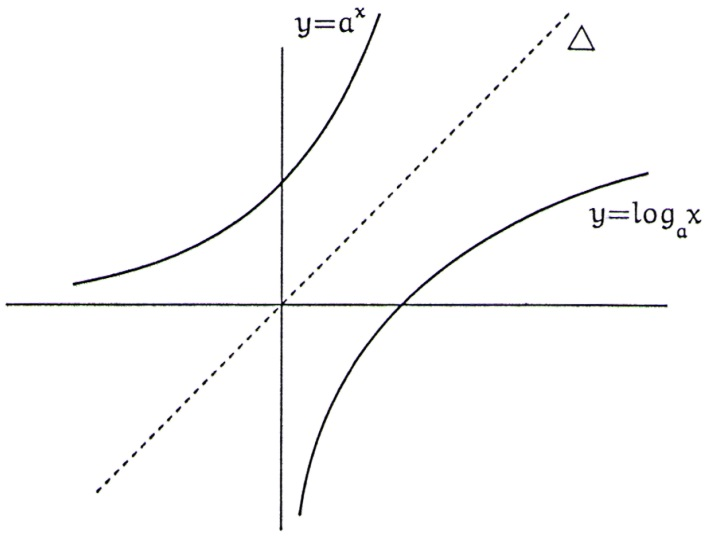
\includegraphics[width=7cm]{figures/logXexp.jpg}
\end{center}


\end{frame}

%------------------------------------------------------------------------------------------------------------
\section{Atividade Online}
\begin{frame}
\frametitle{Atividade Online} %\framesubtitle{Exemplos}

\href{https://pt.khanacademy.org/math/algebra2/exponential-and-logarithmic-functions/graphs-of-logarithmic-functions/e/graphs-of-exponentials-and-logarithms}
{{\tt Atividade 16 - Gráficos de Funções Logarítmicas}}


Veja o desempenho na Missão Álgebra II.


\end{frame}

%------------------------------------------------------------------------------------------------------------
\section{Caracterização da Função Logarítmica}
\begin{frame}
\frametitle{Caracterização da Função Logarítmica} %\framesubtitle{Exemplos}

\begin{Teo}[Caracterização da Função Logarítmica]
Seja $f:  \R_+^\ast \to \R$ uma função monótona injetiva tal que
$f(xy) = f(x) + f(y)$ para quaisquer $x, y \in \R_+^\ast$. Então
existe $a>0$ tal que $f(x) = \log_a x$ para todo $x \in \R_+^\ast$.
\end{Teo}



\end{frame}






%------------------------------------------------------------------------------------------------------------


\section{O número $e$}
\begin{frame}
\frametitle{O número $e$} %\framesubtitle{Exemplos}

\begin{Def}
Definimos o número $e$ como sendo o número cujos valores aproximados
por falta são os números racionais da forma $$
\paren{1+ \frac 1 n}^n , n\in \N^\ast.$$ Em outras palavras, quanto
maior for $n \in \N^\ast$, melhor a aproximação de $\paren{1+ \frac
1 n}^n$ para $e$, e ela se dá na medida que desejarmos.
\end{Def}

\end{frame}

%------------------------------------------------------------------------------------------------------------



\begin{frame}
\frametitle{O número $e$} %\framesubtitle{Exemplos}

O número $e$ é irracional. Um valor aproximado dessa importante
constante é $e = 2{,}718281828459$.

Muito usado como base das funções exponenciais e logarítmicas,
principalmente no estudo dessas funções no Cálculo Infinitesimal, o
logaritmo na base $e$ recebe uma notação e nomenclatura especial.
Denotamos $$\log_e x = \ln x$$ e o chamamos de \sub{logaritmo
natural}.


\end{frame}



%------------------------------------------------------------------------------------------------------------
\section{Atividade Online}
\begin{frame}
\frametitle{Atividade Online} %\framesubtitle{Exemplos}

\href{https://pt.khanacademy.org/math/algebra2/exponential-and-logarithmic-functions/solving-exponential-equations-with-logarithms/e/using-logarithms-to-solve-exponential-equations}
{{\tt Atividade 17 - Solução de Equações Exponenciais Usando
Logaritmos: Base 10 e Base $e$}}


\href{https://pt.khanacademy.org/math/algebra2/exponential-and-logarithmic-functions/solving-exponential-models/e/exponential-models-word-problems}
{{\tt Atividade 18 - Problemas com Modelos Exponenciais}}

Veja o desempenho na Missão Álgebra II.


\end{frame}


%------------------------------------------------------------------------------------------------------------

\section{Exercícios}
\begin{frame}
\frametitle{Exercícios} %\framesubtitle{Exemplos}
\Ex{Mostre que a função $f: \Z \to \R$ definida por $f(x)=a^x$ é
crescente se $a>1$ e decescente se $0<a<1$.}

\Ex{Mostre que a função $f: \Q \to \R$ definida por $f(x)=a^x$ é
crescente se $a>1$ e decescente se $0<a<1$.}

\Ex{Uma alga cresce de modo que, em cada dia, ela cobre uma
superfície de área igual ao dobro da coberta no dia anterior. Se
esta alga cobre a superfície de um lago em 100 dias, qual é o número
de dias necessários para que duas algas, da mesma espécie anterior,
cubram a superfície do mesmo lago? E se forem quatro algas? Você
consegue responder esta pergunta para 3 algas?}

\Ex{O gordinho Jaguatirica, certo dia, fez compras em 5 lojas de um
shopping. Em cada loja, gastou metade do que possuia e pagou, na
saída, R\$ 2{,}00 de estacionamento. Se após toda essa atividade
ainda ficou com R\$ 20{,}00, que quantia ele tinha inicialmente?}

\end{frame}


%------------------------------------------------------------------------------------------------------------

\begin{frame}
\frametitle{Exercícios} %\framesubtitle{Exemplos}

\Ex{Se $\paren{a_n}$ é uma PA, prove que $\paren{ b_n}$ definida por
$b_n = e^{a_n}$ é uma PG.}

\Ex{Existe exemplo de função crescente $f : \N \to \R_+^\ast$ tal
que, para todo $x \in \N$, a sequência $f(x)$, $f(x+1)$, $f(x+2)$,
..., $f(x+n)$, ... é uma progressão geométrica mas $f$ não é do tipo
$f(x) = b \cdot a^x$?}

\end{frame}


%------------------------------------------------------------------------------------------------------------

\begin{frame}
\frametitle{Exercícios} %\framesubtitle{Exemplos}

\Ex{Use as aproximações $\log 2 \approx 0,301$, $\log 3 \approx
0,477$ e $\log 5 \approx 0,699$ para obter valores aproximados para:
\begin{enumerate}[(a)]
	\item $\log 9$;
	\item $\log 40$;
	\item $\log 200$;
	\item $\log 3000$;
	\item $\log 0{,}003$;
	\item $\log 0{,}81$.
\end{enumerate}
}



%\Ex{Dada as PA's $\paren{a_1, a_2, \dots, a_n, \dots}$ e
%$\paren{b_1, b_2, \dots, b_n, \dots}$, mostre que existe uma, e
%somente uma, função afim $f: \R \to \R$ tal que $f(a_1) = b_1$,
%$f(a_2) = b_2$, \dots , $f(a_n) = b_n$, \dots}
\end{frame}

%------------------------------------------------------------------------------------------------------------

\begin{frame}
\frametitle{Exercícios} %\framesubtitle{Exemplos}

\Ex{Uma interpretação do logaritmo decimal é sua relação com a
\sub{ordem de grandeza}, isto é, com o número de algarismos na
representação decimal. As questões a seguir exploram essa relação.
\begin{enumerate}[(a)]
	\item Considere o número $x = 58.932{,}1503$. Qual é a parte inteira de $\log x$?
	\item Considere $x>1$ um número real cuja parte inteira tem $k$ algarismos.
	Use que a função logarítmica é crescente para mostrar que a parte inteira
	de $\log x$ é igual a $k-1$;
	\item Generalizando o item anterior, considere o sistema de
	numeração posicional de base $b \geq 2$. Mostre que, se a
	representação de um número real $x>1$ nesse sistema tem $k$
	algarismos, então, a parte inteira de $\log_b x$ é igual a $k-1$.
\end{enumerate}}


\end{frame}


%------------------------------------------------------------------------------------------------------------

\begin{frame}
\frametitle{Exercícios} %\framesubtitle{Exemplos}

\Ex{(UNIRIO/1994) Um explorador descobriu, na selva amazônica, uma
espécie nova de planta e, pesquisando-a durante anos, comprovou que
o seu crescimento médio variava de acordo com a fórmula $A = 40
\cdot 1{,}1^t$, onde a altura média $A$ é medida em centímetros e o
tempo $t$ em anos. Sabendo-se que $\log 2 \approx 0{,}30$ e $\log 11
\approx 1{,}04$, determine:
\begin{enumerate}[(a)]
	\item A altura média, em centímetros, de uma planta dessa espécie
	aos 3 anos de vida;
	\item A idade, em anos, na qual a planta tem uma altura média de
	$1{,}6 m$.
\end{enumerate}
}



\end{frame}



%------------------------------------------------------------------------------------------------------------

\begin{frame}
\frametitle{Exercícios} %\framesubtitle{Exemplos}

\Ex{Considere $x, y \in \R$ tais que $x = 10^k y$, com $k\in \Z$.
Qual é a relação entre $\log x $ e $\log y$?}

\Ex{Se $\paren{a_n}$ é uma PG com todos os termos positivos, prove
que $\paren{ b_n}$ definida por $b_n = \ln{a_n}$ é uma PA.}

\Ex{O acidente do reator nuclear de Chernobyl, URSS, em 1986, lançou
na atmosfera grande quantidade do isótopo radioativo estrôncio-90,
cuja meia-vida (tempo necessário para que uma substância seja
reduzida à metade da quantidade inicial) é de vinte e oito anos, ou
seja, sendo $f$  a função exponencial de base $a$ que modele a
quantidade de estrôncio-90 em função do tempo, tem-se $\log_a \frac
{f(0)} 2 = 28$. Supondo ser este isótopo a única contaminação
radioativa e sabendo que o local poderá ser considerado seguro
quando a quantidade de estrôncio-90 se reduzir, por desintegração, a
$\frac 1 {16}$ da quantidade inicialmente presente, em que ano o
local poderá ser habitado novamente? }




\end{frame}



%------------------------------------------------------------------------------------------------------------
\begin{comment}
\begin{frame}
\frametitle{Exercícios - Desafios} %\framesubtitle{Exemplos}

\Ex{Seja $f: X \to Y$ uma função. Mostre que, se existem $g_1 : Y
\to X$ e $g_2 : Y \to X$ tais que $f \circ g_1 = \I_Y$ e $g_2 \circ
f = \I_X$, então $g_1 = g_2$ (portanto, neste caso, $f$ será
invertível).}

\Ex{Seja $f: X \to Y$ uma função. Mostre que
\begin{enumerate}[(a)]
	\item $f(f^{-1}(B)) \subset B$, para todo $B \subset Y$;
	\item $f(f^{-1}(B)) = B$, para todo $B \subset Y$ se, e
	somente se, $f$ é sobrejetiva.
\end{enumerate}}

\Ex{Seja $f: X \to Y$ uma função. Mostre que
\begin{enumerate}[(a)]
	\item $f(f^{-1}(A)) \supset A$, para todo $A \subset X$;
	\item $f(f^{-1}(A)) = A$, para todo $A \subset X$ se, e
	somente se, $f$ é injetiva.
\end{enumerate}}

\Ex{Mostre que existe uma injeção $f: X \to Y$ se, e somente se,
existe uma sobrejeção $g: Y \to X$.}

\end{frame}

\end{comment}

%------------------------------------------------------------------------------------------------------------
\begin{comment}
\begin{frame}
\frametitle{Exercícios} %\framesubtitle{Exemplos}





%EXERCÍCIOS PARA FUNÇÕES EXPONENCIAIS E LOGARÍTMICAS
%\Ex{Se $\paren{a_n}$ é uma PG de termos positivos, prove que
%$\paren{ b_n}$ definida por $b_n = \log a_n$ é uma PA.}

%\Ex{Se $\paren{a_n}$ é uma PA, prove que $\paren{ b_n}$ definida por
%$b_n = e^{a_n}$ é uma PG.}
\end{frame}

\end{comment}

%------------------------------------------------------------------------------------------------------------

\begin{comment}
\subsection{Exemplo de uma figura}

\begin{frame}{Título do slide}
\framesubtitle{Sub-título do slide}
\transdissolve
	\includegraphicscopyright[width=6cm]{Figuras/teste.jpg}
	{Copyright by Sir Silva}
\end{frame}
\end{comment}

%------------------------------------------------------------------------------------------------------------


\section{Bibliografia}

\frame{
\frametitle{Bibliografia}

\begin{thebibliography}{99}

\bibitem {label1}
LIMA, Elon L; CARVALHO, Paulo César P; Wagner, Eduardo; MORGADO,
Augusto C.
\newblock {\em A Matemática do Ensino Médio. Vol. 1}.
\newblock 9. ed. Rio de Janeiro: SBM, 2006.

\bibitem {label2}
IEZZI, Gelson; et al.
\newblock {\em Fundamentos de Matemática Elementar. Vol. 2 - Logaritmos}.
\newblock São Paulo: Editora Atual.

%LIMA, Elon L; CARVALHO, Paulo César P; Wagner, Eduardo; MORGADO,
%Augusto C.
%\newblock {\em A Matemática do Ensino Médio. Vol. 2}.
%\newblock 5. ed. Rio de Janeiro: SBM, 2004.

%\bibitem {label1}
%OLIVEIRA, Krerley I M; FERNÁNDEZ, Adán J C.
%\newblock {\em Estágio dos Alunos Bolsistas - OBMEP 2005 - 4. Equações, Inequações e Desigualdades}.
%\newblock Rio de Janeiro: SBM, 2006.

%\bibitem {label2}
%OLIVEIRA, Krerley I M; FERNÁNDEZ, Adán J C.
%\newblock {\em Iniciação à Matemática: um Curso com Problemas e Soluções}.
%\newblock 2. ed. São Paulo: Cengage Learning, 2010.


\end{thebibliography}
}


%------------------------------------------------------------------------------------------------------------


%{\aauwavesbg
%\begin{frame}[plain,noframenumbering]
%  \finalpage{Thank you for using this theme!}
%\end{frame}}
%%%%%%%%%%%%%%%%%

\end{document}
